%%%%%%%%%%%%%%%%%%%%%%%%%%%%%%%%%%%%%%%%%%%%%%%%%%%%%%%%%%%%%%%%%%%%%%%
%%%%  Load the document class and packages                         %%%%
%%%%%%%%%%%%%%%%%%%%%%%%%%%%%%%%%%%%%%%%%%%%%%%%%%%%%%%%%%%%%%%%%%%%%%%
\documentclass[a4paper]{report}
\usepackage{epsfig}            % to insert PostScript figures
\graphicspath{ 
  {./figures/} 
}

%Change figure names
\renewcommand{\figurename}{Fig}

\usepackage[bf,footnotesize]{caption} % make captions small and label bold


\addtocounter{chapter}{1} %Because starting at zero is silly
\makeatletter
\renewcommand{\thesection}{\@arabic\c@section}
\renewcommand{\thefigure}{\@arabic\c@figure}
\makeatother

\usepackage[a4paper,margin=2.7cm,tmargin=2.5cm,bmargin=2.5cm]{geometry} 
\usepackage{textcomp}          % To make nice degree symbols and others\usepackage[bf,footnotesize]{caption} % make captions small and label bold
\usepackage{wrapfig}
%to produce the clickable references along the left in Acroread. This
%package must be included last. 
\usepackage[ps2pdf,bookmarks=TRUE]{hyperref} 



%%%%%%%%%%%%%%%%%%%%%%%%%%%%%%%%%%%%%%%%%%%%%%%%%%%%%%%%%%%%%%%%%%%%%%%
%%%%  Hypertext references for Acrobat                             %%%%
%%%%%%%%%%%%%%%%%%%%%%%%%%%%%%%%%%%%%%%%%%%%%%%%%%%%%%%%%%%%%%%%%%%%%%%
\hypersetup{
pdfauthor = {SWC},
pdftitle = {Optics Exercises},
pdfkeywords = {optics, lenses, refraction, reflection, dispersion,
  telescope, microscope},
pdfcreator = {LaTeX with hyperref},
pdfproducer = {dvips + ps2pdf}
           }


\begin{document}




%set the number of sectioning levels 
\setcounter{secnumdepth}{2}

\begin{center}
\textbf{\Large{Compound Lenses \& Optical Aberrations}}
\end{center}

You should already be familiar with the ray diagram for a telescope (Fig.~\ref{fig:telescope}) and how it works to magnify distant objects. 
This is a `real' ray tracing diagram generated using the professional ray tracing software, Zemax. 
The lenses are both compound lenses. 
Why is this?

\begin{figure}[h]
\center
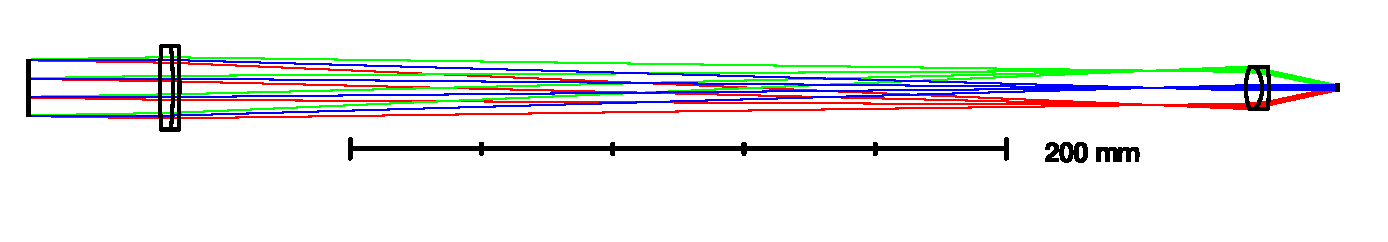
\includegraphics[width=6in]{Telescope.eps}
\caption{A beam expander composed of an $f=300~mm$ lens and an $f=25~mm$ lens. 
In addition to the collimated beam arriving on-axis (blue), two off-axis beams are shown in different colors.
Note how the angles of the beams leaving the $f=25~mm$ are substantially larger.}
\label{fig:telescope}
\end{figure}

\begin{wrapfigure}{R}{0.22\textwidth}
  \begin{center}
    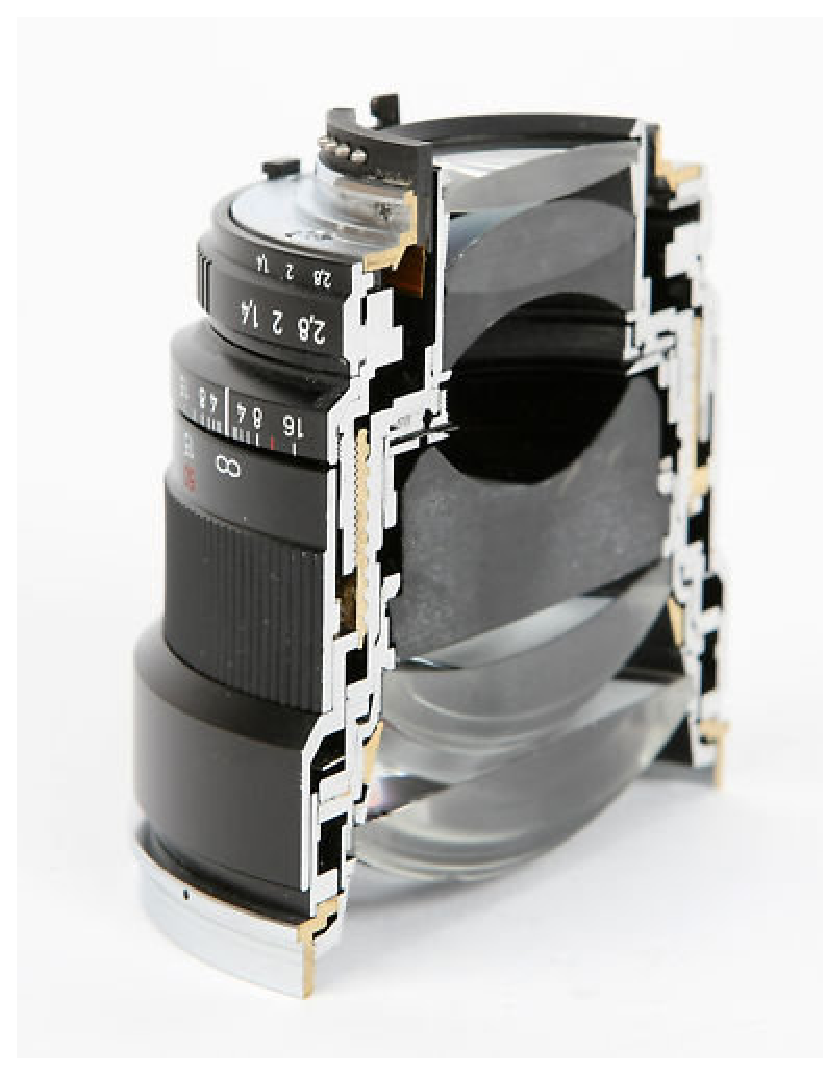
\includegraphics[width=0.22\textwidth]{SLR_lens_cut_in_half.eps}

  \end{center}
  \vspace{-100pt} 
\end{wrapfigure}
In this optional exercise you'll explore image aberrations and see why camera lenses, microscope objectives, and eyepieces contain multiple lenses spaced closely together. 
You will do this by building a variety of simple telescopes and assessing their image quality.
After this exercise you will have learned:
\begin{itemize}
    \setlength\itemsep{0.15em}
    \item Why thin lens ray tracing does not capture aberrations.
    \item What is chromatic aberration and how it can be corrected.
    \item What are spherical aberration (SA) and coma.
    \item How aberrations can be reduced by using smaller ray angles.
\end{itemize}


\subsubsection{Limitations of the thin lens approximation}
The ray tracing you've learned is good for planning simple optical systems but offers no information about image quality. 
This is because your ideal `thin lenses' always observe the image forming condition: all rays leaving a point on the sample plane converge onto a point on the image plane. 
In reality the image forming condition does not always hold. 
Rays hitting the lens at steeper angles will come into focus at a position other than that predicted by thin lens ray tracing. 
This is worse for steeper ray angles and more curved lenses. 
Image `\textbf{aberrations}' occur when rays leaving a point in the sample do not all converge in the image plane.
Rays instead converge in different locations according to a systematic pattern which depends upon the form of the aberration. 
The the three most common aberrations are chromatic aberration, spherical aberration, and coma (Fig.~\ref{fig:aberrations}). 

\begin{figure}[h]
\center
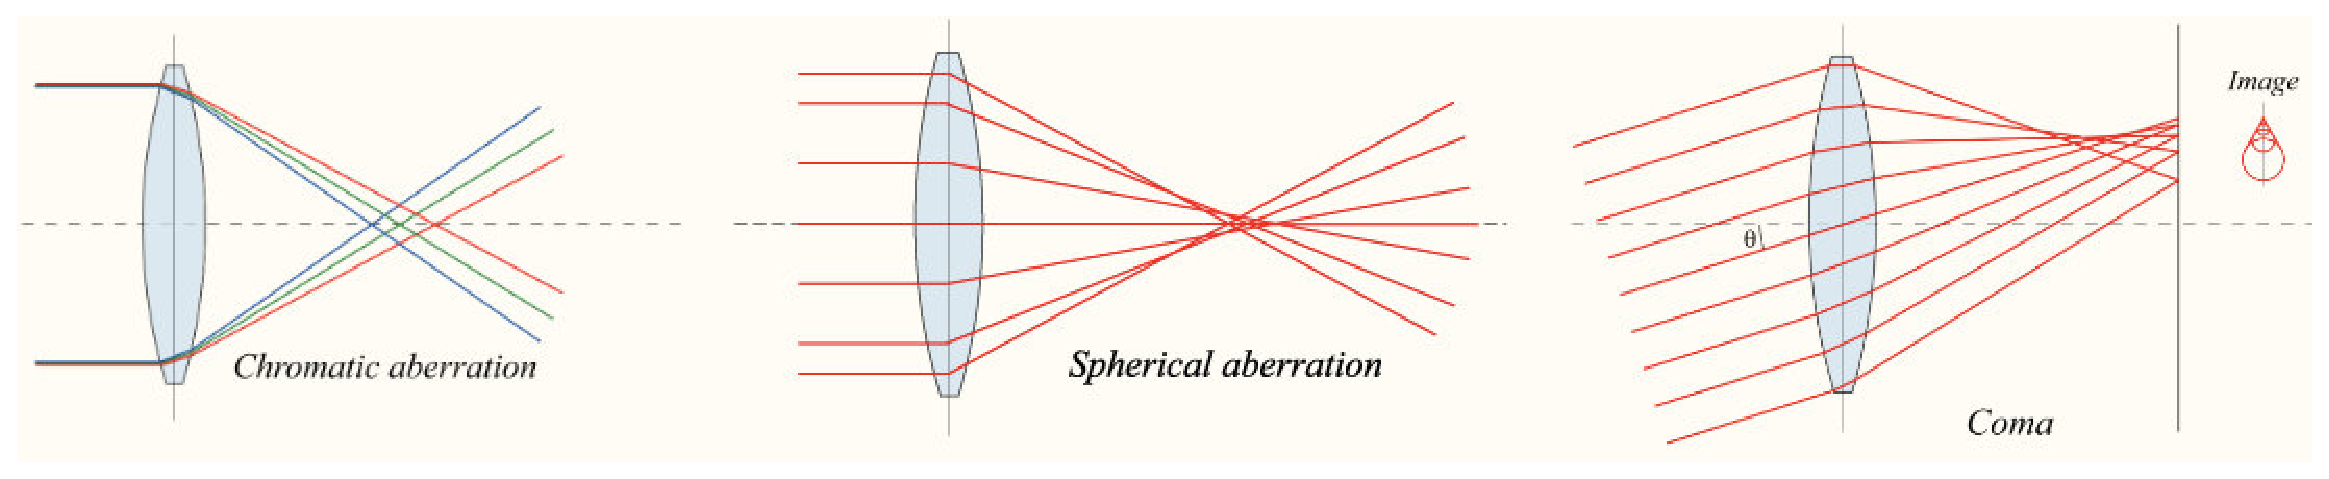
\includegraphics[width=6in]{aberrations.eps}
\caption{ 
Chromatic aberration sees light of different wavelengths coming into focus at different distances from the lens.
Spherical aberration sees on-axis light (that parallel to the optical axis) having different focal lengths depending upon distance from the optical axis. 
Coma is the situation where off-axis light does not come into focus in the same spot. Coma does not occur for rays traveling along the optical axis.}
\label{fig:aberrations}
\end{figure}



\subsubsection{Chromatic aberration}
Blue light is refracted more strongly than red light and so the focal length of a lens is wavelength dependent. 
Lenses therefore have shorter focal lengths for blue light than red light (Fig.~\ref{fig:aberrations}).
This leads to a pronounced wavelength-dependent blurring of the image known as chromatic aberration. 
You will now build a telescope on the 500 mm optical rail:
\begin{itemize}
\item Use an f=300~mm for the objective and an f=25~mm for the eyepiece. 
\item Look through your telescope at an object across the room. How does the chromatic aberration manifest itself?
\item Ask for the f=300~mm achromat and swap your singlet lens with this. Observe the image again.
\end{itemize}

\textbf{How does it work?} 
The first element of the achromat is a positive lens that will converge light. 
The second element is a negative lens that will diverge light.
This second element has a lower power and so together the elements of the achromat constitute a positive lens. 
The two elements are made of glass with different indexes of refraction. 
The second (negative) element has a stronger index of refraction. 
Thus, the second lens diverges blue light more strongly than the first lens can focus it.
This balancing act is finely tuned to bring red and blue light into focus at the same spot.

Coarsely speaking, the second lens of the achromatic doublet disperses light in the \textit{opposite direction} to the first lens in order to bring different wavelengths into a common focus. 
\textbf{Aberrations are generally corrected by adding an element which introduces the opposite aberration.}






\subsubsection{Spherical Aberration \& Coma and Ray Angles}
Look through your telescope and pay attention to how the image quality varies across the field of view. 
What do you see?
What you see is likely due to various different aberrations. 
Let's try to clean up the image. 

Examine Fig.~\ref{fig:aberrations}, whilst it doesn't show how SA and coma arise it does allow us to predict that these aberrations will be less prominent if the outer rays are removed. 
Place an iris on a rail carriage and locate it around 15 cm behind the objective lens. 
Close the iris whilst looking through the telescope. 
As the iris closes, fine features at the edges of the field will become sharper but the field of view doesn't change. 




\subsubsection{Compound Eyepieces}
Using an iris (known as a `pupil') to reduce ray angles is a common approach for taming aberrations but it is limited since it of course also reduces light. 
A better approach is to choose lenses such that you avoid introducing aberrations in the first place. 
You will now replace the $f=25~mm$ lens with a compound lens of similar focal length (Eq.~\ref{eq:compoundLensF} shows how to calculate the effective focal length of two thin lenses separated in air by some distance $d$). 
A compound lens is one where the optical elements are spaced closely together. 
Ask for one of the two compound lenses: one is is composed of two plano-convex singlet lenses (Fig.~\ref{fig:composite}, right)
and the other is known as a Pl\"{o}ssl eyepiece, which is composed of two closely spaced achromats. 
In what ways has the image improved compared to the single $f=25~mm$ lens?
Is the Pl\"{o}ssl better than the singlet pair?

\begin{equation}
\frac{1}{f} = \frac{1}{f_1} + \frac{1}{f_2} - \frac{d}{f_1f_2}
\label{eq:compoundLensF}
\end{equation}


\begin{figure}[h]
\center
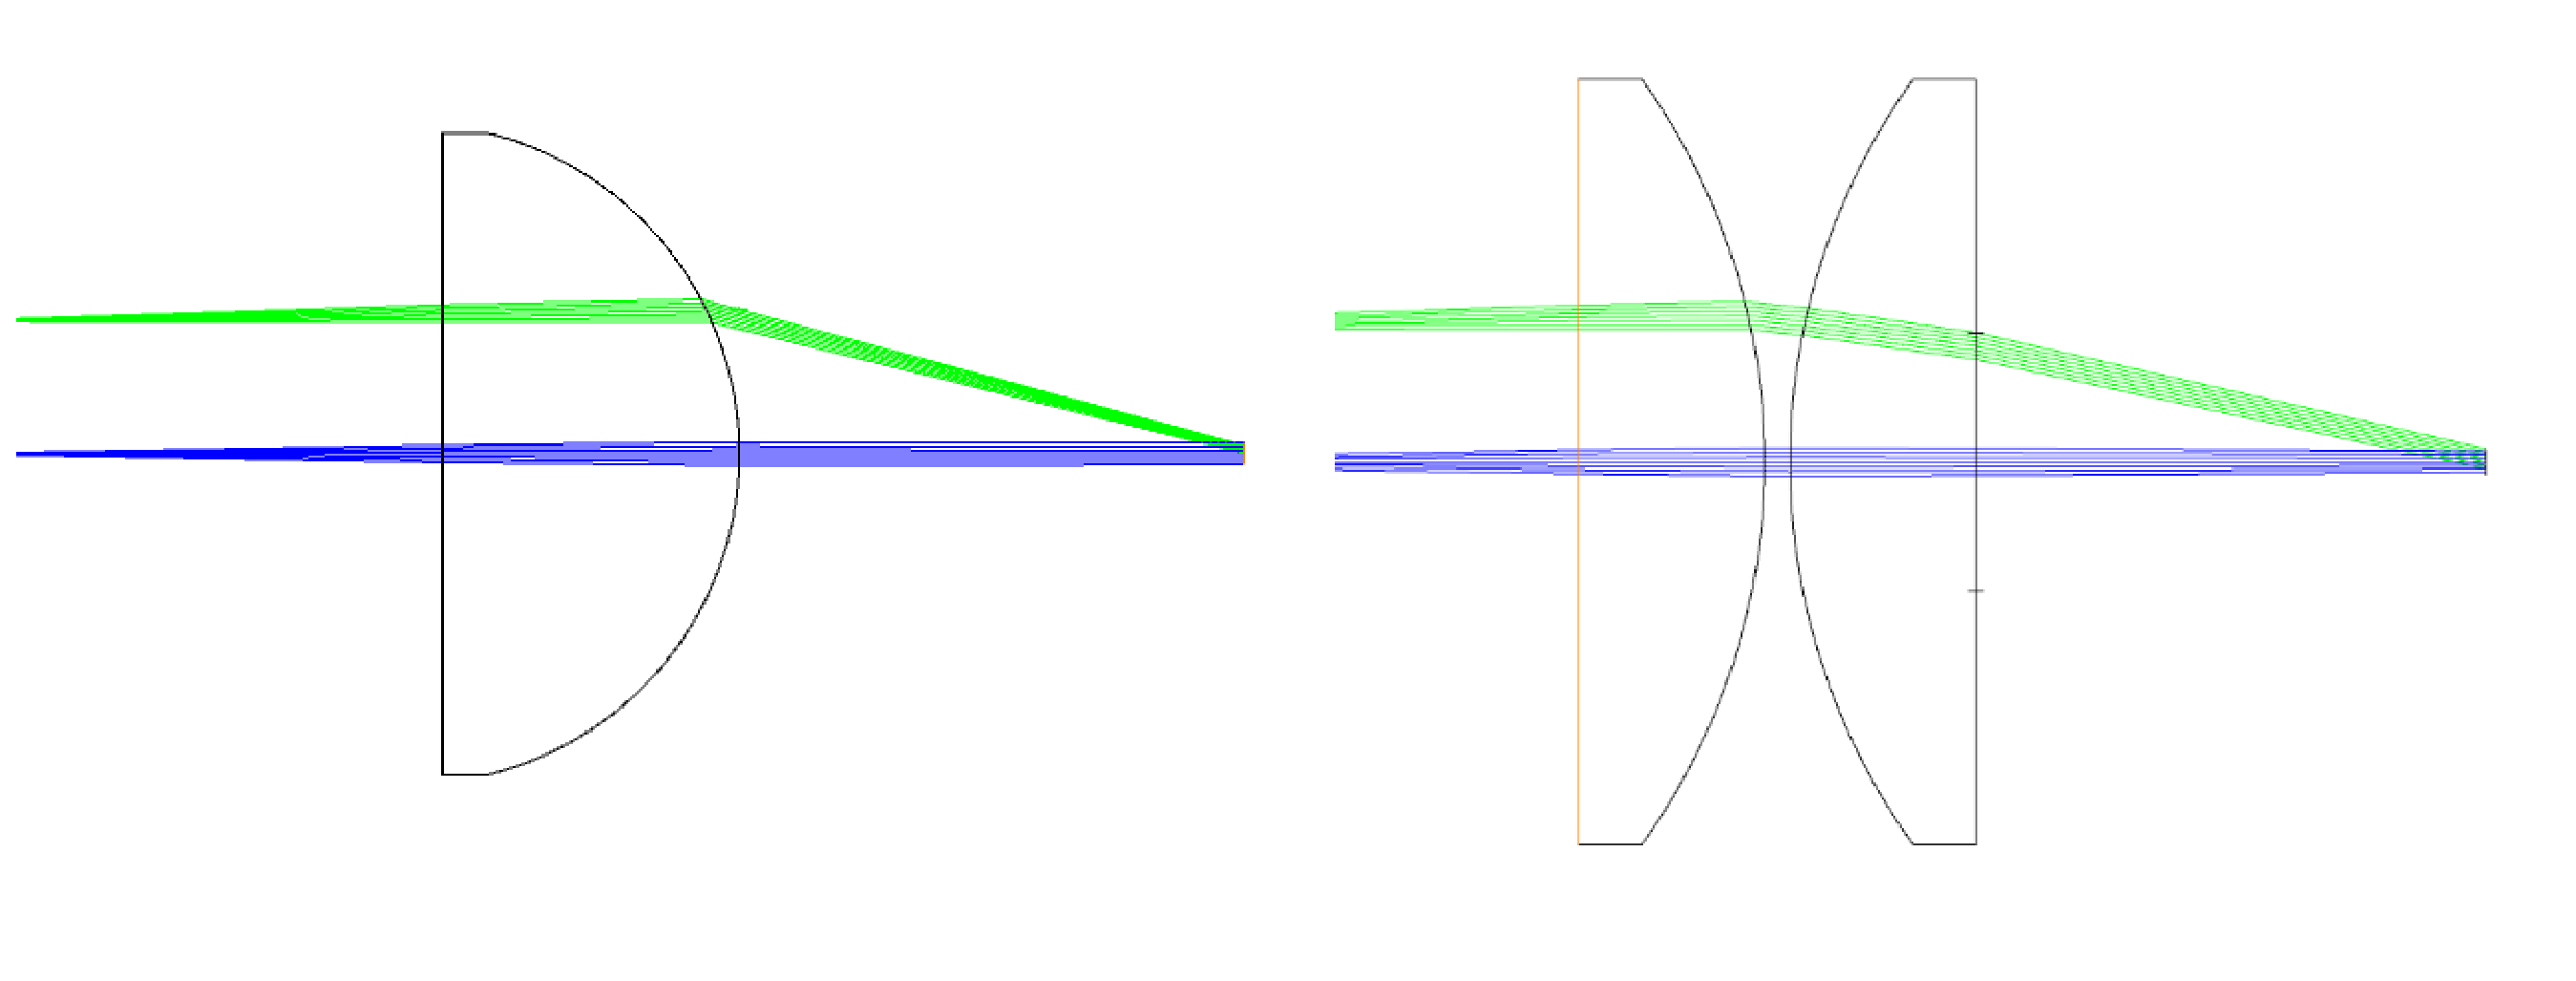
\includegraphics[width=4.5in]{eyepiece_compare.eps}
\caption{Ray diagrams of two of the eyepieces you have access to. Left: $f=25~mm$ plano-convex singlet (you might have a bi-convex version). 
Right: $f=25~mm$ compound lens composed of two $f=50~mm$ singlet lenses. 
Blue rays are on-axis. 
Green rays arise from an object 1 degree off-axis. }
\label{fig:composite}
\end{figure}


\textbf{Why does the compound lens clean up the image edges?} 
The simple answer is that the singlet lens must bend off-axis light by a large amount as it exits (Fig.~\ref{fig:composite}) and this is sufficient to induce large aberrations. 
Even in this low resolution ray diagram, you can see that the green ray is not collimated upon exiting the lens.
The doublet lens spreads the `work' across more surfaces and so avoids introducing aberrations. 
The green rays leaving the final surface remain collimated. 



\end{document}
